\documentclass[autodetect-engine,dvi=dvipdfmx,ja=standard,a4j,jbase=10.5pt,twoside,twocolumn,magstyle=nomag*]{bxjsarticle}
% \documentclass[uplatex, dvipdfmx, a4j, 10ptj, twoside, twocolumn]{jsarticle}
% small japanese font size:     9pt, 10pt, 11pt, 12pt, 14pt, ... (please refer the document of jsclasses)
% word-like japanese font size: 10ptj 10.5ptj, 11ptj, 12ptj (or jbase=xxpt (without 'j') if error is occured)

\RequirePackage{ifptex,ifxetex,ifluatex}
\ifluatex
    \usepackage{bxcalcux}
    \ltjsetparameter{jacharrange={-2,-3}}
    \usepackage{luatexja-otf}
    \usepackage{bxbase}
\else\ifxetex
        % \usepackage{zxjatype}
        % \usepackage[macros]{zxotf}
        \XeTeXgenerateactualtext=1
        \usepackage{xltxtra}
        \usepackage{bxbase}
    \else\ifuptex
            \usepackage{otf}
            \usepackage[prefernoncjk]{pxcjkcat}
            \cjkcategory{sym11,sym18,sym19}{cjk}
            \usepackage[utf8]{inputenc}
            \usepackage{pxbase}
        \else\ifstrictptex
                \usepackage{otf}
                \usepackage[utf8]{inputenc}
                \usepackage{pxbase}
            \fi\fi\fi\fi

\usepackage[LGR,T2A,T1]{fontenc}

% graphic setting (xcolor?)
\usepackage[dvipdfmx]{graphicx, color}

\usepackage{grffile}
% paper layout setting
\usepackage{setspace}

% font setting
\usepackage{amsmath, amssymb}
\usepackage{newtxtext}
\usepackage[slantedGreek]{newtxmath}
\usepackage{mathtools}
\usepackage{bm}
\usepackage{fix-cm}

% caption setting
\usepackage[font=bf,labelfont=bf,labelsep=quad]{caption}

% title font style
\renewcommand{\headfont}{\bfseries}


% line skip setting

% a) basic english lineskip (for article, )
% \narrowbaselines

% b) basic japanese lineskip
% \widebaselines

% c) double-spaced japanese lineskip (= 2 * basic english lineskip)
\narrowbaselines
\usepackage{setspace}
\doublespacing
% \onehalfspacing

% d) others using setspace package
% \usepackage{setspace}
% \setstretch{1.3}
% \setstretch{1.5}

% e) othes using latex command \baselinestretch
% \renewcommand{\baselinestretch}{1.3}
% \renewcommand{\baselinestretch}{1.5}


% header and footer setting
% \usepackage{fancyhdr}
% \makeatletter
% \renewcommand{\chapter}{%
%   \if@openright\cleardoublepage\else\clearpage\fi
%   \global\@topnum\z@
%   \secdef\@chapter\@schapter}
% \makeatother
% \addtolength{\headheight}{\baselineskip}
% \lhead[]{}
% \rhead[\rightmark]{\rightmark}
% \cfoot[\thepage]{\thepage}
% \pagestyle{fancy}


% table of contents setting
\setcounter{tocdepth}{3}
\setcounter{secnumdepth}{3}

% Command             10pt    11pt    12pt
% \tiny               5       6       6
% \scriptsize         7       8       8
% \footnotesize       8       9       10
% \small              9       10      10.95
% \normalsize         10      10.95   12
% \large              12      12      14.4
% \Large              14.4    14.4    17.28
% \LARGE              17.28   17.28   20.74
% \huge               20.74   20.74   24.88
% \Huge               24.88   24.88   24.88

\newcommand{\kintou}[2]{%
    \leavevmode
    \hbox to #1{%
        \setkanjiskip{0truept plus 1fill minus 1fill}
        \setxkanjiskip{\getkanjiskip}
        #2%
    }}

\newcommand{\spacedjpbox}[2]{%
    \leavevmode
    \mbox{%
        \setkanjiskip{#1 plus 0truept minus 0truept}
        \setxkanjiskip{\getkanjiskip}
        #2%
    }}

\ifluatex
    \usepackage{lltjext}
    %
\else\ifptex
        \usepackage{plext}
        \usepackage{plextarray}
        \usepackage{plextdelarray}
        %
    \fi\fi

% for creating graphic elements
\usepackage{tikz}

% e-TeX tools
\usepackage{etoolbox}

\newcommand{\circled}[2][]{%
    \tikz[baseline=(char.base)]{%
        \node[shape = circle, draw, inner sep = 1pt]
        (char) {\phantom{\ifblank{#1}{#2}{#1}}};%
        \node at (char.center) {\makebox[0pt][c]{#2}};}}
\robustify{\circled}


\makeatletter
%
\newcommand*{\years}[1]{\gdef\@years{#1}}
% \newcommand*{\adviser}[1]{\gdef\@adviser{#1}}
% \newcommand*{\adviserposition}[1]{\gdef\@adviserposition{#1}}
\newcommand*{\department}[1]{\gdef\@department{#1}}
\newcommand*{\fieldandcourse}[1]{\gdef\@fieldandcourse{#1}}
%
\newcommand*{\spinetitle}[1]{\gdef\@spinetitle{#1}}
\newcommand*{\spineyears}[1]{\gdef\@spineyears{#1}}
\newcommand*{\spinedepartment}[1]{\gdef\@spinedepartment{#1}}
\newcommand*{\spinefieldandcourse}[1]{\gdef\@spinefieldandcourse{#1}}
\newcommand*{\spinedepartmentfoot}[1]{\gdef\@spinedepartmentfoot{#1}}
%
%
\renewcommand{\maketitle}{%
    %
    \begin{titlepage}%
        %
        % \newgeometry{left=15truemm,right=15truemm}%
        \centering%
        %
        \vfil%
        %
        \begin{minipage}[c][0.2\textheight][c]{\textwidth}%
            \centering%
            \onehalfspacing%
            {\fontsize{29.86truept}{29.86truept}\selectfont\mcfamily%
                \@title%
                \par}%
        \end{minipage}%
        %
        \vspace{0.35\textheight}%
        \vfil%
        %
        \begin{minipage}[c][0.1\textheight][c]{\textwidth}%
            \centering%
            {\fontsize{24.88truept}{24.88truept}\selectfont%
                \@years%
                \par}%
        \end{minipage}%
        %
        \vspace{0.05\textheight}%
        \vfil%
        %
        \begin{minipage}[c][0.3\textheight][c]{\textwidth}%
            \centering%
            \singlespacing%
            {\fontsize{24.88truept}{24.88truept}\selectfont\spacedjpbox{2.49truept}{%
                    \@department%
                }\par}%
            %\vspace{24.88truept}%
            {\fontsize{24.88truept}{24.88truept}\selectfont\spacedjpbox{2.49truept}{%
                    \@fieldandcourse%
                }\par}%
            \vspace{49.76truept}%
            % {\fontsize{24.88truept}{24.88truept}\selectfont\kintou{0.4\textwidth}{%
            {\fontsize{24.88truept}{24.88truept}\selectfont\spacedjpbox{18.66truept}{%
                    \@author%
                }\par}%
        \end{minipage}%
        %
        \vfil%
        %
        % \restoregeometry%
        %
    \end{titlepage}%
}
%
%
\newcommand{\makespinebase}{%
    %
    \begin{tabular}{|c|}%
        %
        \begin{minipage}[c][287truemm][c]{10truemm}%
            \centering%
            %
            \vfil%
            %
            % year number
            \begin{minipage}[c][12truemm][c]{\textwidth}%
                \centering%
                {\fontsize{10truept}{10truept}\selectfont%
                    \circled[00000]{\@spineyears}%
                }%
            \end{minipage}%
            %
            \vfil%
            %
            \ifxetex
                %
                \rotatebox{-90}{%
                    \defaultfontfeatures{Vertical=RotatedGlyphs,RawFeature={vertical}}%
                    \begin{minipage}[c][\textwidth][c]{60truemm}%
                        \raggedright%
                        \doublespacing%
                        {\fontsize{10truept}{10truept}\selectfont\spacedjpbox{1.0truept}{%
                                \@spinedepartment%
                            }\par}%
                        {\fontsize{10truept}{10truept}\selectfont\spacedjpbox{1.0truept}{%
                                \@spinefieldandcourse%
                            }\par}%
                    \end{minipage}%
                    \defaultfontfeatures{Vertical=ResetAll,RawFeature={}}%
                }%
                %
                \vfil%
                %
                \rotatebox{-90}{%
                    \defaultfontfeatures{Vertical=RotatedGlyphs,RawFeature={vertical}}%
                    \begin{minipage}[c][\textwidth][c]{125truemm}%
                        \raggedright%
                        \onehalfspacing%
                        {\fontsize{10truept}{10truept}\selectfont%
                            \@spinetitle%
                            \par}%
                    \end{minipage}%
                    \defaultfontfeatures{Vertical=ResetAll,RawFeature={}}%
                }%
                %
                \vfil%
                %
                \rotatebox{-90}{%
                    \defaultfontfeatures{Vertical=RotatedGlyphs,RawFeature={vertical}}%
                    \begin{minipage}[c][\textwidth][c]{45truemm}%
                        \raggedleft%
                        {\fontsize{10truept}{10truept}\selectfont\spacedjpbox{5.0truept}{%
                                \@author%
                            }\par}%
                    \end{minipage}%
                    \defaultfontfeatures{Vertical=ResetAll,RawFeature={}}
                }%
                %
            \else
                %
                \begin{minipage}<t>[c][\textwidth][c]{60truemm}%
                    \raggedright%
                    \doublespacing%
                    {\fontsize{10truept}{10truept}\selectfont\spacedjpbox{1.0truept}{%
                            \@spinedepartment%
                        }\par}%
                    {\fontsize{10truept}{10truept}\selectfont\spacedjpbox{1.0truept}{%
                            \@spinefieldandcourse%
                        }\par}%
                \end{minipage}%
                %
                \vfil%
                %
                \begin{minipage}<t>[c][\textwidth][c]{125truemm}%
                    \raggedright%
                    \onehalfspacing%
                    {\fontsize{10truept}{10truept}\selectfont%
                        \@spinetitle%
                        \par}%
                \end{minipage}%
                %
                \vfil%
                %
                \begin{minipage}<t>[c][\textwidth][c]{45truemm}%
                    \raggedleft%
                    {\fontsize{10truept}{10truept}\selectfont\spacedjpbox{5.0truept}{%
                            \@author%
                        }\par}%
                \end{minipage}%
            \fi
            %
            \vspace*{25truemm}%
            \vfil%
            %
            \begin{minipage}[c][20truemm][c]{\textwidth}%
                \centering%
                \onehalfspacing
                {\fontsize{10truept}{10truept}\selectfont%
                    \@spinedepartmentfoot%
                    \par}%
            \end{minipage}%
            %
            \vfil%
            %
        \end{minipage}%
        % }
    \end{tabular}%
    %
}
%
%
\newcommand{\makespineonce}{%
    \begin{titlepage}%
        %
        \newgeometry{top=4truemm,bottom=4truemm,left=5truemm,right=5truemm}%
        %textheight = 297mm - 8mm = 289mm -> spine: 287mm
        %
        \vfil%
        %
        \makespinebase%
        %
        \vfil%
        %
        \restoregeometry%
        %
    \end{titlepage}%
}
%
%
\newcommand{\makespine}[1][5]{%
    \begin{titlepage}%
        \newgeometry{top=4truemm,bottom=4truemm,left=5truemm,right=5truemm}%
        \vfil%
        %
        \newcount\cntspine%
        \newcount\cntmax%
        \cntspine=1%
        \cntmax=#1%
        \advance\cntmax-1%
        \loop%
        \makespinebase%
        \hspace{10truemm}%
        \advance\cntspine1%
        \ifnum\cntspine<\cntmax \repeat%
        %
        \makespinebase%
        \vfil%
        \restoregeometry%
    \end{titlepage}%
}
%
%
\makeatother

% load thesis info
\title{射影変換とStyle Transferを用いた\\デザイン文字列作成法に関する研究}
\author{馬場 将史} % please use full-width space in japanese name
\years{令和4年度}
\department{大阪市立大学工学部}
\fieldandcourse{電気情報工学科}

\spinetitle{射影変換とStyle Transferを用いたデザイン文字列作成法に関する研究}
\spineyears{4}
\spinedepartment{大阪市立大学工学部}
\spinefieldandcourse{工学部電気情報工学科}
\spinedepartmentfoot{工学部}

% load cumstom preamble
% % 多言語対応 default languageを指定しないと勝手に英語化されたりする
% \usepackage{ifptex,ifxetex,ifluatex}
% \ifluatex
%     \usepackage{polyglossia}
%     \setdefaultlanguage{japanese}
%     \setotherlanguages{english,russian,greek}
%     % \newfontfamily\greekfont{Liberation Sans}[Mapping=tex-text]
%     % \newfontfamily\greekfontsf{Liberation Serif}[Mapping=tex-text]
%     % \newfontfamily\cyrillicfont{CMU Serif}[Script=Cyrillic,Mapping=tex-text]
%     % \newfontfamily\cyrillicfontsf{CMU Sans Serif}[Script=Cyrillic,Mapping=tex-text]
% \else\ifxetex
%         \usepackage{polyglossia}
%         \setdefaultlanguage{japanese}
%         \setotherlanguages{english,russian,greek}
%         % \newfontfamily\greekfont{Liberation Sans}[Mapping=tex-text]
%         % \newfontfamily\greekfontsf{Liberation Serif}[Mapping=tex-text]
%         % \newfontfamily\cyrillicfont{CMU Serif}[Script=Cyrillic,Mapping=tex-text]
%         % \newfontfamily\cyrillicfontsf{CMU Sans Serif}[Script=Cyrillic,Mapping=tex-text]
%     \else\ifuptex
%             \usepackage[korean,schinese,tchinese,greek,russian,english,japanese]{pxbabel} % for greek, russian
%         \else\ifstrictptex
%                 \usepackage[korean,schinese,tchinese,greek,russian,english,japanese]{pxbabel} % for greek, russian
%             \fi\fi\fi\fi

% for conditional commands
\usepackage{ifthen}

% for bibliography
\usepackage[backend=biber,style=ieee]{biblatex}
\ExecuteBibliographyOptions{mincitenames=1,maxcitenames=1}
% for separate compilation
\usepackage{subfiles}

% set paths using \homedir for separate compilation
\graphicspath{
    {\homedir/figures/},
    {\homedir/figures/chapter1/},
    {\homedir/figures/chapter2/},
    {\homedir/figures/chapter3/},
    {\homedir/figures/chapter4/},
    {\homedir/figures/chapter5/},
}
\addbibresource{\homedir/reference.bib}

\newboolean{printBibInSubfiles}
\setboolean{printBibInSubfiles}{true}
\newcommand{\printBibForSubfiles}{
    \ifthenelse{\boolean{printBibInSubfiles}}
    {
        \printbibliography[title=参考文献]
    }{}
}

% table and array
\usepackage{array}
\usepackage{booktabs}   % \toprule, \midrule, \bottomrule in tabbler environment (with good spacing)
\usepackage{longtable}
% \usepackage{tabularx}
% \usepackage{ltablex}
% \renewcommand{\arraystretch}{0.5}
% \renewcommand{\doublerulesep}{1pt}

% caption
\usepackage{subcaption}
\captionsetup{compatibility=false}

% for algorithm
\usepackage{algorithm,algpseudocode}

\renewcommand{\algorithmicrequire}{\textbf{Input:}}
\renewcommand{\algorithmicensure}{\textbf{Output:}}
\algnewcommand{\algorithmicand}{\textbf{ and }}
\algnewcommand{\algorithmicor}{\textbf{ or }}

\algnewcommand{\OR}{\algorithmicor}
\algnewcommand{\AND}{\algorithmicand}
\algnewcommand{\Countinue}{\textbf{countinue}}
\algnewcommand{\Break}{\textbf{break}}
\algnewcommand{\LeftComment}[1]{\Statex \(\triangleright\) #1}

% extend enumarate
\usepackage{enumitem}

% misc
% \usepackage[hyphens]{url}
% \usepackage{siunitx} %for SI unit


% \usepackage{minted} % pip install --user pygments %for code

% in­tel­li­gent cross-ref­er­enc­ing
%\crefname{env name}{singular}{plural}
% usage:
% in middle of line: \cref{<label>}, \cref{<label1>,<label2>,...} 
% at head of line:   \Cref{<label>}, \Cref{<label1>,<label2>,...} 
\usepackage[capitalise,noabbrev]{cleveref}
% for japanese
\crefformat{chapter}{#2{第}#1{章}#3}
\crefformat{section}{#2#1{}節#3}
\crefformat{subsection}{#2#1{}節#3}
\crefname{figure}{図}{図}
\crefname{table}{表}{表}
\crefname{equation}{式}{式}
\crefname{appendix}{付録}{付録}
\newcommand{\crefrangeconjunction}{--}
\newcommand{\crefpairconjunction}{,}
\newcommand{\crefmiddleconjunction}{,}
\newcommand{\creflastconjunction}{,}
\newcommand{\crefpairgroupconjunction}{,}
\newcommand{\crefmiddlegroupconjunction}{,}
\newcommand{\creflastgroupconjunction}{,}
% for english (only figure and table)
% \renewcommand{\figurename}{Fig.~}
% \renewcommand{\tablename}{Table~}
% \crefname{figure}{Fig.}{Figs.}
% \Crefname{figure}{Figure}{Figures}
% \crefname{table}{Table}{Tables}


% math font (integral, summation, product)
\ifptex
    \DeclareSymbolFont{cmlargesymbols}{OMX}{cmex}{m}{n}
    \DeclareMathSymbol{\intop}{\mathop}{cmlargesymbols}{"5A}
    \def\int{\intop\nolimits}
    \DeclareMathSymbol{\ointop}{\mathop}{cmlargesymbols}{"49}
    \def\oint{\ointop\nolimits}
    \DeclareMathSymbol{\sumop}{\mathop}{cmlargesymbols}{"58}
    \let\sum\sumop
    \DeclareMathSymbol{\prodop}{\mathop}{cmlargesymbols}{"59}
    \let\prod\prodop
\fi



% title setting
\title{射影変換とStyle Transferを用いた\\デザイン文字列作成法に関する研究}
\etitle{A Method for Design Text Creation Using Projective Transformation and Style Transfer}

% author setting
% \studentid{A19TN030}
\author{馬場 将史}
\laboarea{情報処理領域}
% \laboname{知識情報処理工学研究室}

\date{}
% % 多言語対応 default languageを指定しないと勝手に英語化されたりする
% \usepackage{ifptex,ifxetex,ifluatex}
% \ifluatex
%     \usepackage{polyglossia}
%     \setdefaultlanguage{japanese}
%     \setotherlanguages{english,russian,greek}
%     % \newfontfamily\greekfont{Liberation Sans}[Mapping=tex-text]
%     % \newfontfamily\greekfontsf{Liberation Serif}[Mapping=tex-text]
%     % \newfontfamily\cyrillicfont{CMU Serif}[Script=Cyrillic,Mapping=tex-text]
%     % \newfontfamily\cyrillicfontsf{CMU Sans Serif}[Script=Cyrillic,Mapping=tex-text]
% \else\ifxetex
%         \usepackage{polyglossia}
%         \setdefaultlanguage{japanese}
%         \setotherlanguages{english,russian,greek}
%         % \newfontfamily\greekfont{Liberation Sans}[Mapping=tex-text]
%         % \newfontfamily\greekfontsf{Liberation Serif}[Mapping=tex-text]
%         % \newfontfamily\cyrillicfont{CMU Serif}[Script=Cyrillic,Mapping=tex-text]
%         % \newfontfamily\cyrillicfontsf{CMU Sans Serif}[Script=Cyrillic,Mapping=tex-text]
%     \else\ifuptex
%             \usepackage[korean,schinese,tchinese,greek,russian,english,japanese]{pxbabel} % for greek, russian
%         \else\ifstrictptex
%                 \usepackage[korean,schinese,tchinese,greek,russian,english,japanese]{pxbabel} % for greek, russian
%             \fi\fi\fi\fi

% for conditional commands
\usepackage{ifthen}

% for bibliography
\usepackage[backend=biber,style=ieee]{biblatex}
\ExecuteBibliographyOptions{mincitenames=1,maxcitenames=1}
% for separate compilation
\usepackage{subfiles}

% set paths using \homedir for separate compilation
\graphicspath{
    {\homedir/figures/},
    {\homedir/figures/chapter1/},
    {\homedir/figures/chapter2/},
    {\homedir/figures/chapter3/},
    {\homedir/figures/chapter4/},
    {\homedir/figures/chapter5/},
}
\addbibresource{\homedir/reference.bib}

\newboolean{printBibInSubfiles}
\setboolean{printBibInSubfiles}{true}
\newcommand{\printBibForSubfiles}{
    \ifthenelse{\boolean{printBibInSubfiles}}
    {
        \printbibliography[title=参考文献]
    }{}
}

% table and array
\usepackage{array}
\usepackage{booktabs}   % \toprule, \midrule, \bottomrule in tabbler environment (with good spacing)
\usepackage{longtable}
% \usepackage{tabularx}
% \usepackage{ltablex}
% \renewcommand{\arraystretch}{0.5}
% \renewcommand{\doublerulesep}{1pt}

% caption
\usepackage{subcaption}
\captionsetup{compatibility=false}

% for algorithm
\usepackage{algorithm,algpseudocode}

\renewcommand{\algorithmicrequire}{\textbf{Input:}}
\renewcommand{\algorithmicensure}{\textbf{Output:}}
\algnewcommand{\algorithmicand}{\textbf{ and }}
\algnewcommand{\algorithmicor}{\textbf{ or }}

\algnewcommand{\OR}{\algorithmicor}
\algnewcommand{\AND}{\algorithmicand}
\algnewcommand{\Countinue}{\textbf{countinue}}
\algnewcommand{\Break}{\textbf{break}}
\algnewcommand{\LeftComment}[1]{\Statex \(\triangleright\) #1}

% extend enumarate
\usepackage{enumitem}

% misc
% \usepackage[hyphens]{url}
% \usepackage{siunitx} %for SI unit


% \usepackage{minted} % pip install --user pygments %for code

% in­tel­li­gent cross-ref­er­enc­ing
%\crefname{env name}{singular}{plural}
% usage:
% in middle of line: \cref{<label>}, \cref{<label1>,<label2>,...} 
% at head of line:   \Cref{<label>}, \Cref{<label1>,<label2>,...} 
\usepackage[capitalise,noabbrev]{cleveref}
% for japanese
\crefformat{chapter}{#2{第}#1{章}#3}
\crefformat{section}{#2#1{}節#3}
\crefformat{subsection}{#2#1{}節#3}
\crefname{figure}{図}{図}
\crefname{table}{表}{表}
\crefname{equation}{式}{式}
\crefname{appendix}{付録}{付録}
\newcommand{\crefrangeconjunction}{--}
\newcommand{\crefpairconjunction}{,}
\newcommand{\crefmiddleconjunction}{,}
\newcommand{\creflastconjunction}{,}
\newcommand{\crefpairgroupconjunction}{,}
\newcommand{\crefmiddlegroupconjunction}{,}
\newcommand{\creflastgroupconjunction}{,}
% for english (only figure and table)
% \renewcommand{\figurename}{Fig.~}
% \renewcommand{\tablename}{Table~}
% \crefname{figure}{Fig.}{Figs.}
% \Crefname{figure}{Figure}{Figures}
% \crefname{table}{Table}{Tables}


% math font (integral, summation, product)
\ifptex
    \DeclareSymbolFont{cmlargesymbols}{OMX}{cmex}{m}{n}
    \DeclareMathSymbol{\intop}{\mathop}{cmlargesymbols}{"5A}
    \def\int{\intop\nolimits}
    \DeclareMathSymbol{\ointop}{\mathop}{cmlargesymbols}{"49}
    \def\oint{\ointop\nolimits}
    \DeclareMathSymbol{\sumop}{\mathop}{cmlargesymbols}{"58}
    \let\sum\sumop
    \DeclareMathSymbol{\prodop}{\mathop}{cmlargesymbols}{"59}
    \let\prod\prodop
\fi

% ##############################################################################
\begin{document}
% title
\maketitle
% ##############################################################################
\section{はじめに}\label{sec:introduction}
現代では,我々はしばしば色やエフェクトなどによって装飾された文字を目にする.
このように装飾された文字は「デザイン文字」と呼ばれる.

デザイン文字は装飾のないシンプルな文字と比べ,
目立ちやすく具体的なイメージを与えやすいという利点がある.
そのため,デザイン文字は特に目立たせたい文字や印象づけたい文字に用いられることが多い.
例えば,作品のタイトル・企業名・商品名などのロゴ,チラシ,ポスター広告などは
印象に残ることが重要なため,よくデザイン文字が用いられている.

一方,デザイン文字作成は高度な技術や多大な時間を要するという欠点がある.
そのため,デザイン文字の簡単な作成手法が求められており,
Style Transferを用いて自動作成する手法が
既にいくつか研究・開発されている~\cite{Yang_2017_CVPR,Yang2019Controllable,typography2019}.

また,「デザイン文字を用いてまで印象を強めたい文字」は,
固有名詞や何かのメッセージのような意味のある文字列の一部であることが多い.
つまり,デザイン文字が用いられる際には単一の文字としてではなく,
複数文字からなる文字列として用いられることが多いと予想できる.

ゆえに,「デザイン文字」の作成手法よりも「デザイン文字列」の作成手法の方が有用だと考え,
「デザイン文字列を自動で作成する手法の開発」を本研究の目的とした.

なお,デザイン文字列には単一の文字からなるデザイン文字では考慮する必要のなかった
デザインの要素がいくつか存在する.
そういった要素の例として,文字の間隔や配置,文字列全体の形状の歪みが挙げられる.
これらの要素はより目を引くデザイン文字列を作成するために用いられる.

こうしたデザイン文字列特有のデザインの要素のうち,
本研究では「文字列全体の形状の歪み」に射影変換や区分線形回帰を用いて対応することを試みた.
先行研究では,デザイン文字列に特有のデザインの要素は注目されて来なかったため,
本研究の試みには新規性があるといえる.

% ##############################################################################
\section{提案手法}\label{sec:methods}
\subsection{対象とするデザイン文字列}
本研究の提案手法では,デザイン文字列のうち文字の配置が横一行のもののみを対象とする.
つまり,\cref{sec:introduction}で述べたようなデザイン文字列特有のデザインの要素のうち,
文字列全体の形状の歪みのみを本手法の対象とし,文字の配置や文字の間隔などは対象外とする.

\subsection{デザイン文字列自動作成の概要}
本研究の提案手法を用いてデザイン文字列を作成するには次の4つの入力データが必要である.

\begin{enumerate}
    \item 使用したい文字列の白黒画像
    \item 形状の歪みを指定するための白黒文字列画像
    \item エフェクトを指定するためのデザイン文字
    \item 入力3のデザイン文字に使用されている文字の形状を示す白黒画像
\end{enumerate}

これらの入力データのうち,入力1と入力2の文字列の文字の配置は横一列とする.
但し,入力2については形状の歪みによる配置のずれがあっても良いとする.
さらに,入力2は次の二つの条件を満たす必要がある.
\begin{enumerate}[label=\textbf{条件\arabic*:}]
    \item 入力2は画像中の適切な位置で,適切な回数だけ,縦線で左右に画像を分割すれば,
          分割された各領域内の形状の歪みは単純な射影変換で再現できる.
    \item 条件1で述べた画像の適切な分割回数は,入力2の文字数に比べて十分少ない.
\end{enumerate}
これらのうち条件1は,
入力2の各文字のバウンディングボックス(以下,B.B.と表記する)の中心座標の横方向成分に対し,
B.B.の中心座標の縦方向成分やB.B.の大きさが区分的にほぼ線形となることを意味する.
また,条件2は形状の歪み方が同じ領域内に文字のB.B.が十分な数存在することを意味する.

\begin{figure}[h]
    \centering
    \begin{minipage}[b]{0.48\linewidth}
        \centering
        
\includegraphics[keepaspectratio, width=0.9\linewidth]{warp_style.png}
        \subcaption{もとの文字列画像}
        \label{fig:warp_style_wo_guide}
    \end{minipage}
    \begin{minipage}[b]{0.48\linewidth}
        \centering
        
\includegraphics[keepaspectratio, width=0.9\linewidth]{warp_style_bb.png}
        \subcaption{各文字のB.B.}
        \label{fig:warp_style_with_bb}
    \end{minipage}
    \\
    \begin{minipage}[b]{0.7\linewidth}
        \centering
        
\includegraphics[keepaspectratio, width=0.9\linewidth]{warp_style_guide.png}
        \subcaption{区分線形性}
        \label{fig:warp_style_with_guide}
    \end{minipage}
    \caption{入力2の条件を満たす文字列画像}
    \label{fig:warp_style}
\end{figure}

例として,\cref{fig:warp_style_wo_guide}の文字列画像を
\cref{fig:warp_style_with_guide}のように「P」の付近で左右に分割することを考える.
このとき分割された各領域内には2文字以上のB.B.が含まれ,
それらのB.B.は中心座標の横方向成分に対して中心座標の縦方向成分や大きさは
ほぼ線形であることが読み取れる.
よって,\cref{fig:warp_style_wo_guide}の文字列画像は入力2の条件を満たす.

このような文字列画像であれば,
\cref{fig:warp_style_wo_guide}のように白黒画像のみしか与えられていない場合でも,
\cref{fig:warp_style_with_bb}のように各文字のB.B.を計算し,
その後適切な区間の分割数で区分線形回帰を行うことで,
形状の歪み方が切り替わる境界および各領域の歪み方に対応する射影変換行列を求められるため,
別の文字列へと文字列の形状の歪みを転写することができる.
次の\cref{fig:warp_transfer_eg}は\cref{fig:warp_style_wo_guide}の文字列画像の歪みを
\cref{fig:content}に実際に転写を行った例である.

\begin{figure}[h]
    \centering
    \begin{minipage}[b]{0.48\linewidth}
        \centering
        
\includegraphics[keepaspectratio, width=0.9\linewidth]{content.png}
        \subcaption{もとの文字列}
        \label{fig:content}
    \end{minipage}
    \begin{minipage}[b]{0.48\linewidth}
        \centering
        
\includegraphics[keepaspectratio, width=0.9\linewidth]{content_warped.png}
        \subcaption{歪みを転写した文字列}
        \label{fig:content_warped}
    \end{minipage}
    \caption{形状の歪みの転写例}
    \label{fig:warp_transfer_eg}
\end{figure}

以上で述べた歪みの転写の実装にはpythonのライブラリのnumpyとOpenCVとpwlfを用いた.

このように歪みを転写することで得られた文字列画像に対し,
先行研究\cite{typography2019}で提案されたモデルを用いて
エフェクトのStyle Transferを行うことで最終的なデザイン文字列を得る.

% ##############################################################################
\section{評価実験}\label{sec:experiment}
\cref{sec:methods}で述べた提案手法の有効性を確かめるために,
同研究室の学生及び情報処理領域の学生を対象にアンケートを実施し,
最終的に十五人から回答を得た.
このアンケートは次の5つのセクションからなる.

\begin{enumerate}
    \item 入力1の文字種による影響の調査
    \item 入力3による影響の調査その1
    \item 入力2の文字種による影響の調査
    \item 入力3による影響の調査その2
    \item 入力2の歪み方による影響の調査
\end{enumerate}

アンケートの各セクションでは調べたいもののみ入力を変え,
各入力が結果に与える影響を調査した.
例えば,セクション1では英大文字,英小文字,漢字の3種で入力1を作成し,
その他の入力は全て変えずにデザイン文字列を作成した上で,
入出力の組み合わせが分かるような画像を回答者に見せてアンケートを取った.

また,入出力の組み合わせ1パターンにつき,次の4つの項目を設けて,
各項目について「全く当てはまらない」を1,「とても当てはまる」を5とした五段階評価のデータをとった.
\begin{enumerate}[label=\textbf{項目\arabic*:}]
    \item resultの色や効果はeffect styleと似ている
    \item resultの文字列の歪みはwarp styleと似た形状である
    \item resultの文字列はcontentの文字列と同じ文字と分かる
    \item resultのデザイン文字列は上手く生成されている
\end{enumerate}

アンケートの評価を各質問の各項目ごとに全回答者の平均値をとったものが
次の\cref{tab:questionnaire}である.
なお,表中の「全」の項目は各質問に対し全項目の平均値を取った値である.

\begin{table}[h]
    \centering
    \caption{アンケート結果}
    \begin{tabular}[t]{ccccccc}
        \toprule
        質問    & 項目1  & 項目2  & 項目3  & 項目4  & 全    \\
        \midrule
        1 - 1 & 4.53 & 4.60 & 4.73 & 4.53 & 4.60 \\
        1 - 2 & 4.07 & 3.07 & 3.40 & 3.07 & 3.40 \\
        1 - 3 & 4.00 & 3.00 & 2.53 & 2.60 & 3.03 \\
        \hline
        2 - 1 & 4.27 & 4.67 & 4.80 & 4.40 & 4.53 \\
        2 - 2 & 4.20 & 4.53 & 4.80 & 4.33 & 4.47 \\
        2 - 3 & 3.93 & 4.53 & 4.73 & 4.07 & 4.32 \\
        2 - 4 & 3.13 & 4.20 & 4.73 & 3.73 & 3.95 \\
        2 - 5 & 3.67 & 4.33 & 4.80 & 4.00 & 4.20 \\
        \hline
        3 - 1 & 4.20 & 3.00 & 4.27 & 3.40 & 3.72 \\
        3 - 2 & 4.47 & 4.20 & 4.67 & 4.13 & 4.37 \\
        3 - 3 & 3.47 & 2.13 & 1.60 & 1.53 & 2.18 \\
        \hline
        4 - 1 & 3.07 & 4.33 & 4.80 & 3.60 & 3.95 \\
        4 - 2 & 4.40 & 4.73 & 4.80 & 4.53 & 4.62 \\
        4 - 3 & 4.07 & 4.67 & 4.73 & 4.13 & 4.40 \\
        4 - 4 & 2.80 & 4.27 & 4.33 & 3.13 & 3.63 \\
        4 - 5 & 2.80 & 4.53 & 4.60 & 3.40 & 3.83 \\
        \hline
        5 - 1 & 4.33 & 4.60 & 4.80 & 4.47 & 4.55 \\
        5 - 2 & 4.53 & 4.67 & 4.87 & 4.67 & 4.68 \\
        5 - 3 & 4.33 & 4.60 & 4.27 & 4.07 & 4.32 \\
        5 - 4 & 4.20 & 3.00 & 4.60 & 3.20 & 3.75 \\
        \bottomrule
    \end{tabular}
    \label{tab:questionnaire}
\end{table}

\cref{tab:questionnaire}の値を見ると評価が4以上である項目が多いことから,
提案したデザイン文字列の作成手法は概ね良い評価を受けているといえる.

その中で,質問3-3は極端に悪い評価を受けているが,これは入力2の文字種を漢字としたものである.
質問3-3の入出力の組み合わせを次の\cref{fig:warp_style_text_kanji}に示すが,
この組み合わせでは文字の歪みの転写に失敗していることが読み取れる.
\begin{figure}[h]
    \centering
    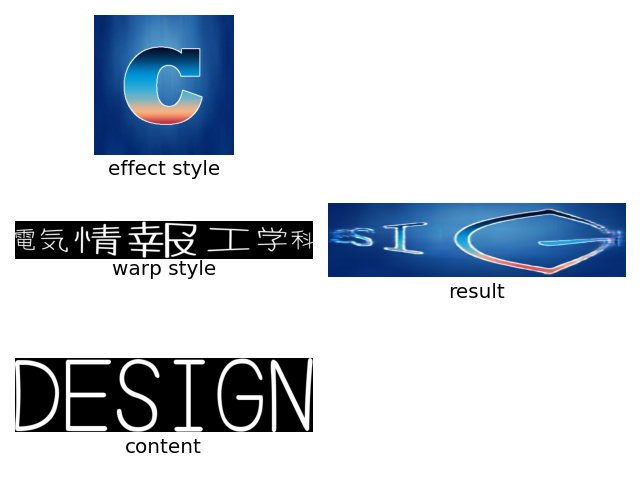
\includegraphics[keepaspectratio, width=0.9\linewidth]{warp_style_text_kanji.png}
    \caption{質問3-3で提示した入出力の組み合わせ}
    \label{fig:warp_style_text_kanji}
\end{figure}

% ##############################################################################
\section{まとめ}\label{sec:summary}
本研究が提案するデザイン文字列の作成手法は概ね有用だと示された.
しかし,歪みを指定する文字列画像に漢字を用いた場合など,
デザイン文字列の作成に失敗する組み合わせも見られたため,
提案手法には改善の余地がある.
% ##############################################################################
% bibliography
\begin{thebibliography}{9}
    \bibitem{Yang_2017_CVPR}Yang, S., Liu, J., Lian, Z. \& Guo, Z. Awesome Typography: Statistics-Based Text Effects Transfer. {\em Proceedings Of The IEEE Conference On Computer Vision And Pattern Recognition (CVPR)}. (2017,7)
    \bibitem{Yang2019Controllable}Yang, S., Wang, Z., Wang, Z., Xu, N., Liu, J. \& Guo, Z. Controllable Artistic Text Style Transfer via Shape-Matching GAN. {\em International Conference On Computer Vision}. (2019)
    \bibitem{typography2019}Wang, W., Liu, J., Yang, S. \& Guo, Z. Typography with Decor: Intelligent Text Style Transfer. {\em The IEEE Conference On Computer Vision And Pattern Recognition (CVPR)}. (2019,6)
\end{thebibliography}
% ##############################################################################
\end{document}
